\vspace{1cm}
\fancyhead[C]{\normalsize\textbf{$\qquad$ Teil I: Offene Aufgaben}}
\renewcommand{\labelenumi}{\theenumi.}
\section*{Aufgabe 1 (35 Punkte)}
\vspace{0.4cm}
\subsection*{\aufgabe{a}{10}}
Swisslos ist in der deutschsprachigen Schweiz staatlicher Monopolist im Bereich Zahlenlottos und Sportwetten und bietet unter anderem die Produkte Swiss Lotto und Euro Millions an.
Bei einem  Verkaufspreis $ x $ pro Los der Sorte (1) Swiss Lotto und einem Verkaufspreis $ y $ pro Los der Sorte (2) Euro Millions lauten die Nachfragefunktionen:
\begin{align*}
\textrm{Nachfrage nach Swiss Lotto:} 
&\quad
q_{d_1}(x,y) = 39'500 - 1'000 x + 400y,\\
\textrm{Nachfrage nach Euro Millions:}
&\quad
q_{d_2}(x,y) = 6'500 + 300 x - 800 y.
\end{align*}
Gesucht sind die Preise $ x $ und $ y $, bei denen der Gesamtumsatz maximal ist.\\
Es wird dabei vorausgesetzt, dass die Nachfragemengen auch abgesetzt werden.\\
\\
Weisen Sie nach, dass es sich wirklich um ein Maximum handelt und berechnen Sie auch den maximalen Umsatz.
\\
\\
\textbf{Lösung:}
\begin{mdframed}
\underline{\textbf{Vorgehensweise:}}
\renewcommand{\labelenumi}{\theenumi.}
\begin{enumerate}
\item Stelle eine mathematische Modellierung auf.
\item Finde die Preise für den maximalen Gesamtumsatz.

\end{enumerate}
\end{mdframed}
\underline{1. Stelle eine mathematische Modellierung auf}\\
Zunächst betrachten wir die Einnahmen der einzelnen Lose.
Die Einnahmen ergeben sich aus dem Produkt des Preises mit der Menge.
Durch $ x $ und $ y $ sind die Preise und durch $ q_1 $ und $ q_2 $ die Mengen gegeben.
Für Swiss Lotto erhalten wir die Einnahmefunktion
\begin{align*}
E_S (x,y) = \underbrace{x}_{\textrm{Preis}} \ \underbrace{q_{d_1}(x,y)}_{\textrm{Menge}}
\end{align*}
und für Euro Millions gilt
\begin{align*}
E_E(x,y) = \underbrace{y}_{\textrm{Preis}} \  \underbrace{q_{d_2}(x,y)}_{\textrm{Menge}}.
\end{align*}
Laut Aufgabenstellung gilt die Annahme, dass die Nachfragemenge auch abgesetzt wird.
Der Gesamtumsatz entspricht der Summe von $ E_S $ und $ E_E $.
Damit gilt 
\begin{align*}
G(x,y)
&=
E_S(x,y) + E_E(x,y) 
= 
x q_{d_1}(x,y) + y q_{d_2}(x,y)\\
&=
x(39'500 - 1'000 x + 400y ) + y (6'500 + 300 x - 800 y)\\
&=
39'500x - 1'000 x^2 + 400 xy + 6'500 y + 300 xy - 800 y^2\\
&=
- 1'000 x^2 - 800 y^2 + 700 xy + 39'500x + 6'500 y
\end{align*}
für den Gesamtumsatz $ G $. Die zu maximierende Zielfunktion ist gefunden. Außerdem sind an die Preise $ x $ und $ y $ keine Nebenbedingungen gesetzt.
Somit lösen wir ein globales Maximierungsproblem, d.h. wir betrachten eine Extremwertaufgabe ohne Nebenbedingungen.\\
\\
\underline{2. Finde die Preise für den maximalen Gesamtumsatz}\\
Da wir keine Nebenbedingungen vorliegen haben, betrachten wir die partiellen Ableitungen:
\begin{align*}
G_x(x,y) &= -2'000 x + 700 y + 39'500\\
G_y(x,y) &= -1'600 y + 700 x + 6'500.
\end{align*}
Ein Extremum kann nur vorliegen, falls
\begin{align*}
G_x(x,y) &= -2'000 x + 700 y + 39'500 = 0  \ \Leftrightarrow \ -2'000 x + 700 y  = -39'500 \ \Leftrightarrow \ -20 x + 7 y  = -395\\
G_y(x,y) &= -1'600 y + 700 x + 6'500 = 0  \ \Leftrightarrow \ -1'600 y + 700 x  = - 6'500 \ \quad  \Leftrightarrow \ -16 y + 7 x  = - 65.
\end{align*}
erfüllt ist. Die Lösung des linearen Gleichungsystems erhalten wir durch Anwendung des Gauß Algorithmus mit:
\begin{align*}
\begin{gmatrix}[p]
-20 & 7 & \BAR & -395\\
7 & -16 & \BAR & -65
\rowops
\mult{0}{\cdot 7}
\mult{1}{\cdot 20}
\end{gmatrix} 
&\leadsto
\begin{pmatrix}
-140 & 49 & \BAR & -395 \cdot 7\\
140 & -320 & \BAR & -65 \cdot 20
\end{pmatrix}
=
\begin{pmatrix}
-140 & 49 & \BAR & -2765\\
140 & -320 & \BAR & -1300
\end{pmatrix}\\
&\leadsto
\begin{pmatrix}
-140 & 49 & \BAR & -2765\\
0 & -271 & \BAR & -4065
\end{pmatrix}
\leadsto
\begin{pmatrix}
-140 & 49 & \BAR & -2765\\
0 & 1 & \BAR & \frac{4065}{271}
\end{pmatrix}
=
\begin{pmatrix}
-140 & 49 & \BAR & -2765\\
0 & 1 & \BAR & 15
\end{pmatrix}\\
&\leadsto
\begin{pmatrix}
-140 & 0 & \BAR & -2765 - 
49 \cdot 15\\
0 & 1 & \BAR & 15
\end{pmatrix}
=
\begin{pmatrix}
-140 & 0 & \BAR & -3500\\
0 & 1 & \BAR & 15
\end{pmatrix}\\
&\leadsto
\begin{pmatrix}
1 & 0 & \BAR & \frac{3500}{140}\\
0 & 1 & \BAR & 15
\end{pmatrix}
=
\begin{pmatrix}
1 & 0 & \BAR & 25\\
0 & 1 & \BAR & 15
\end{pmatrix}
\end{align*} 
Die partiellen Ableitungen $ G_x $ und $ G_y $ sind also für $ (x_0,y_0) = (25,15) $ null.
Wir haben also genau einen Kandidaten für ein Extremum gefunden und müssen überprüfen von welcher Art dieser Kandidat ist.\\
\\
Die Bedingung für ein Maximum ist durch
\begin{align*}
G_{xx}(x_0,y_0) < 0 \wedge G_{yy}(x_0,y_0) < 0 \wedge
G_{xx}(x_0,y_0) \cdot G_{yy}(x_0,y_0) - (G_{xy}(x_0,y_0))^2 > 0
\end{align*}
gegeben. Die partiellen Ableitung der zweiten Ordnung sind durch 
\begin{align*}
G_{xx}(x,y) &= -2'000 = G_{xx}(x_0,y_0)\\
G_{yy}(x,y) &= -1'600 = G_{yy}(x_0,y_0)\\
G_{xy}(x,y) &= G_{yx}(x,y) = + 700 =  G_{xy}(x_0,y_0)  
\end{align*}
gegeben. Damit gilt unmittelbar $ G_{xx}(x_0,y_0) < 0 $ und $ G_{yy}(x_0,y_0) <0 $.
Einsetzen in den letzten Teil der Bedingung liefert uns 
\begin{align*}
G_{xx}(x_0,y_0) \cdot G_{yy}(x_0,y_0) - (G_{xy}(x_0,y_0))^2
=
(-2'000) \cdot (- 1'600) - (700)^2
=
2'000 \cdot 1'600 - 700^2  > 0. 
\end{align*}
Also liegt an der Stelle $ (x_0,y_0 ) = (25,15) $ ein Maximum vor und die maximalen Einnahmen sind durch 
\begin{align*}
G(25,15) = - 1'000\cdot (25)^2 - 800 \cdot  (15)^2 + 700 \cdot 25 \cdot 15 + 39'500\cdot 25 + 6'500 \cdot 15=
... 
=
542'500 \ CHF
\end{align*}
gegeben.
\newpage

\subsection*{\aufgabe{b}{10}}
Gesucht ist der Punkt $ P = (x^\ast,y^\ast) $ mit $ x^\ast > 0  $ und $ y^\ast > 0 $ auf der Kurve
\begin{align*}
\varphi(x,y) = 
cx^2 +(1-c) y^2 -2 = 0, \textrm{ wobei } c \in \mathbb{R} \textrm{ mit } 0 < c < 1,
\end{align*}
sodass das Rechteck mit achsenparallelen Seiten, einer Ecke im Punkt $ (0,0) $ und der gegenüberliegenden Ecke in $ P = (x^\ast, y^\ast) $ maximale Fläche hat.\\
\\
Ermitteln Sie Kandidaten $ (x^\ast, y^\ast) $ für mögliche Maxima in Abhängigkeit des Parameters $ c $.\\
\\
\textit{Wichtige Bemerkung:}\\
Eine Abklärung, ob es sich bei den potentiellen Kandidaten um Extremstellen handelt und von welcher Art (Maxima und Minima) sie sind, wird \textbf{nicht} verlangt.
\\ \\
\textbf{Lösung:}
\begin{mdframed}
\underline{\textbf{Vorgehensweise:}}
\renewcommand{\labelenumi}{\theenumi.}
\begin{enumerate}
\item Bestimme die Art der Kurve.
\item Stelle das Problem grafisch dar.
\item Stelle das Extremwertproblem auf.
\item Löse das Extremwertproblem. 
\end{enumerate}
\end{mdframed}

\underline{1. Gebe das durch die Kurve beschriebene geometrische Objekt an und schränke es passend ein}\\
Für die Kurve $ \varphi $ gilt
\begin{align*}
\varphi(x,y) = cx^2 +(1-c) y^2 -2 = 0
&\ \Leftrightarrow \
c x^2 + (1-c) y^2 = 2\\
&\ \Leftrightarrow \
c \frac{x^2}{2} + (1-c) \frac{y^2}{2} = 1 \\
&\ \Leftrightarrow \
 \frac{x^2}{\frac{2}{c}} +  \frac{y^2}{\frac{2}{1-c}}
 = 1\\
&\ \Leftrightarrow \
 \frac{x^2}{\left(\sqrt{\frac{2}{c}}\right)^2} +  \frac{y^2}{\left(\sqrt{\frac{2}{1-c}}\right)^2}
  = 1
\end{align*}
für $ 0 < c < 1 $. Damit beschreibt sie eine Ellipse mit den Halbachsen $ a = \sqrt{\frac{2}{c}} $ und $ b = \sqrt{\frac{2}{1-c}} $. 
\newpage
\underline{2. Stelle das Problem grafisch dar}\\
Die Grafik
\begin{center}
	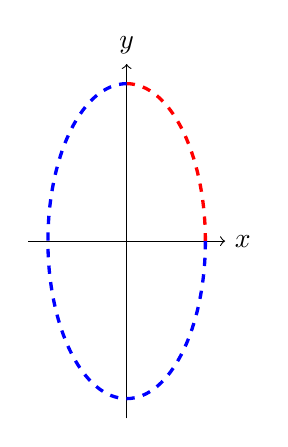
\begin{tikzpicture}[scale=0.5]
	%\draw[help lines, color=gray!30, dashed] (-2.9,-2.9) grid (4.9,4.9);
	\draw[->] (-2.5,0)--(2.5,0) node[right]{$x$};
	\draw[->] (0,-4.5)--(0,4.5) node[above]{$y$};
	\draw[very thick,dashed,red] (0,4) arc(90:180:-2cm and 4cm);
	\draw[very thick,dashed,blue] (2,0) arc(180:450:-2cm and 4cm);
	\end{tikzpicture}
\end{center}
stellt die Ellipse schematisch dar. Da der gesuchte Punkt $ P = (x^\ast,y^\ast) $ auf der Kurve $ \varphi(x,y) = 0 $ mit $ x^\ast, y^\ast > 0 $ liegt, befindet sich der relevante Kurventeil im ersten Quadraten der Grafik.
Dies ist an der roten Markierung erkennbar.\\
Die Eckpunkte $ (0,0)  $ und $ (x^\ast, y^\ast) $ bilden ein achsenparalleles Rechteck.
Damit sind die anderen beiden Eckpunkte durch $ (0,y^\ast) $ und $ (x^\ast,0) $ gegeben. Das Rechteck lässt sich folgendermaßen visualisieren:
\begin{center}
	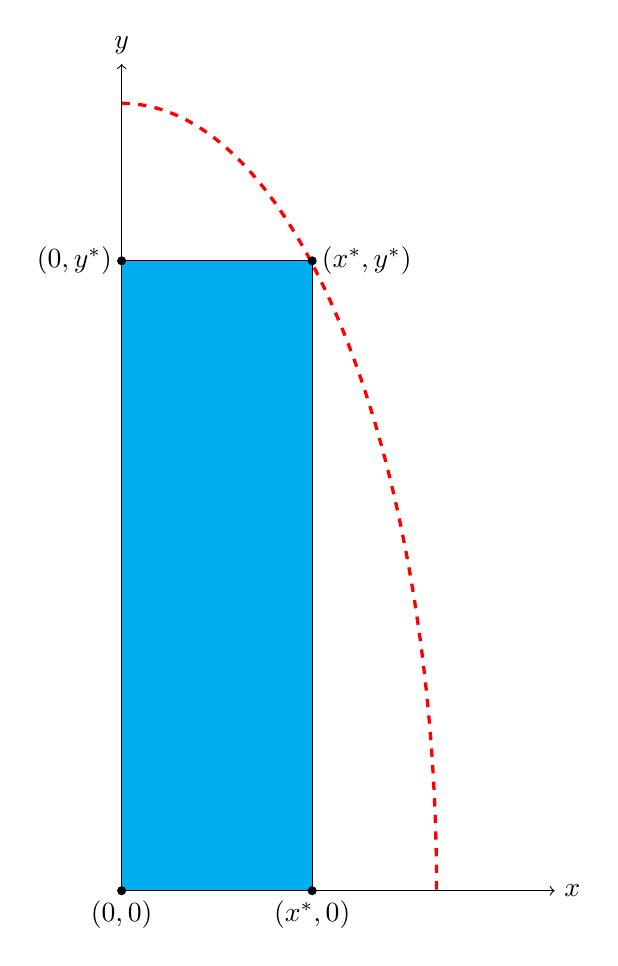
\begin{tikzpicture}
	%\draw[help lines, color=gray!30, dashed] (-2.9,-2.9) grid (4.9,4.9);
	\draw[->] (0,0)--(5.5,0) node[right]{$x$};
	\draw[->] (0,0)--(0,10.5) node[above]{$y$};
	\draw[very thick,dashed,red] (0,10) arc(90:180:-4cm and 10cm);
	
	\filldraw[draw=black,fill=cyan] (0,0) rectangle (2.42,8);
	\draw[fill] (2.42,8) circle [radius=0.05cm];
	\draw[fill] (0,8) circle [radius=0.05cm];
	\draw[fill] (2.42,0) circle [radius=0.05cm];
	\draw[fill] (0,0) circle [radius=0.05cm];
	\node[right] at (2.42,8) {$ (x^\ast, y^\ast) $};
	\node[left] at (0,8) {$ (0, y^\ast) $};
	\node[below] at (0,0) {$ (0, 0) $};
	\node[below] at (2.42,0) {$ (x^\ast, 0) $};
	\end{tikzpicture}
\end{center}

\newpage
\underline{3. Stelle das Extremwertproblem auf}\\
%Unser Ziel ist nun den Flächeninhalt des Rechtecks zu maximieren, wobei $ (x^\ast, y^\ast) $ die Nebenbedingung $ \varphi $ erfüllen muss. Hiermit liegt ein Extremwertproblem unter Nebenbedingungen vor.
Die Zielfunktion ist durch 
\begin{align*}
f(x,y) = x \cdot y
\end{align*}
gegeben. Für $ x,y > 0 $ beschreibt diese den Flächeninhalt eines Rechtecks mit den Seiten $ x $ und $ y $.
Unser Ziel ist es, Kandidaten für mögliche Extremstellen von $ f $ unter der Nebenbedingung
\begin{align*}
\varphi(x,y) = 
cx^2 +(1-c) y^2 -2 = 0
\end{align*}
zu finden.\\
\\
\underline{4. Löse das Extremwertproblem}\\
Die erste Möglichkeit ist die Lagrange-Methode. Hierfür definieren wir die Lagrangefunktion:
\begin{align*}
F(x,y, \lambda ) = f(x,y) + \lambda \varphi(x,y)
= xy + \lambda(c x^2 + (1-c)y^2 -2 ).
\end{align*}
Notwendig für Extremstellen von $ f $ unter der Nebenbedingung $ \varphi(x,y)= 0 $ ist, dass die partiellen Ableitungen der Lagrangefunktion gleich null sind.
Durch Differenzieren und Gleichsetzen erhalten wir:
\begin{align*}
F_x(x,y, \lambda) = y + 2\lambda  c^2 x \qquad \qquad \   &\ \Rightarrow \ y + 2\lambda  c x = 0  \ 
\qquad \qquad \quad  \textrm{(I)}\\
F_y(x,y,\lambda) = x + 2 \lambda (1-c) y \qquad \  &\ \Rightarrow \ x + 2 \lambda (1-c) y = 0\  \quad \quad \  \textrm{(II)}\\
F_\lambda(x,y,\lambda) = c x^2 +(1-c) y^2 -2 &\ \Rightarrow \  c x^2 +(1-c) y^2 -2= 0\  \textrm{(III)}.
\end{align*}
Zunächst konzentrieren wir uns auf die Gleichungen (I) und (II).
Für die erste beiden Gleichungen gilt:
\begin{align*}
y  + 2 \lambda c x = 0 \ \Leftrightarrow \
y = - 2 \lambda c x \quad \textrm{und} \quad 
x + 2 \lambda (1-c) y = 0  \Leftrightarrow \ x = - 2 \lambda (1-c) y
\end{align*}
Wir dividieren $ y $ mit $ x  $ und erhalten:
\begin{align*}
\frac{y}{x} = 
\frac{- 2 \lambda c x}{- 2 \lambda (1-c) y}
=
\frac{cx}{(1-c)y} = \frac{c}{1-c} \cdot \frac{x}{y}
\ \Leftrightarrow \
y = 
\frac{c}{1-c} \cdot \frac{x^2}{y}
\ \Leftrightarrow 
y^2 = \frac{c}{1-c} x^2.
\end{align*}
In die Gleichung (III) eingesetzt liefert dies mit $ 0 < c < 1 $:
\begin{align*}
 c x^2 +(1-c) y^2 -2 &= 
 c x^2 +(1-c) \cdot \frac{c}{1-c} x^2 -2
 =
 c x^2 + c x^2 - 2 = 2 c x^2 - 2 = 0\\
 \ &\Leftrightarrow \
 2c x^2= 2 \\
 \ &\Leftrightarrow \
 x^2 = \frac{2}{2c}= \frac{1}{c}
\ \Rightarrow \
 x = \pm \sqrt{\frac{1}{c}} 
.
\end{align*}
Da $ x > 0  $ vorausgesetzt sind, erhalten wir $ x = \frac{1}{\sqrt{c} } $.
Wenn wir $ x $ in den Ausdruck $ y^2 = \frac{c}{1-c} x^2 $ einsetzen folgt wegen $ y >0 $:
\begin{align*}
y^2 = \frac{c}{1-c} \left( \frac{1}{\sqrt{c}}\right)^2 = \frac{1}{1-c} 
\ \Rightarrow \
y = \frac{1}{\sqrt{1-c}}. 
\end{align*}

Damit ist ein eindeutiger Kandidat $ (x^\ast,y^\ast) = \left(\frac{1}{\sqrt{c}  },  \frac{1}{\sqrt{1-c}}\right) $ für eine Extremstelle gefunden.\\
\\
\ \\ 
Alternativ lässt sich die Nebenbedingung mit unseren Voraussetzungen durch
\begin{align*}
\varphi(x,y) = cx^2 +(1-c) y^2 -2 = 0 
\ \Leftrightarrow \
y^2 = \frac{2 - cx^2}{1-c}
\ \overset{y > 0}{\Leftrightarrow} \
y(x) =  \sqrt{\frac{2 - cx^2}{1-c}}
\end{align*}
als Funktion darstellen. 
Unser Extremwertproblem reduziert sich dann auf die Bestimmung der kritischen Stellen des eindimensionalen Problems
\begin{align*}
A(x) = x y(x).
\end{align*}
Sei $ x_0 $ eine kritische Stelle von $ A $. Dann ist $ (x_0,y(x_0)) = (x_0,y_0) $ ein Kandidat für eine Extremstelle unseres Ausgangsproblem.  
\newpage
\subsection*{\aufgabe{c}{5}}
Für eine Person, die am t.m.j geboren ist, sei der \glqq Geburtstagsvektor\grqq \ $ \textbf{g} = 
\begin{pmatrix}
t \\ m \\ j
\end{pmatrix}
$.
Zum Beispiel ist der Geburtstagsvektor von Leonhard Euler, der am 15. April 1707 geboren wurde, $ \textbf{e}
=
\begin{pmatrix}
15 \\ 4 \\ 1707
\end{pmatrix}
$.
Gegeben sind die Geburtstagsvektoren von
\begin{align*}
&\textrm{Hermann Grassmann } 
\textbf{g}_1 =
\begin{pmatrix}
15 \\ 4 \\ 1809
\end{pmatrix}\\
&\textrm{William Hamilton } 
\textbf{h} =
\begin{pmatrix}
8 \\ 3 \\ 1788
\end{pmatrix}\\
&\textrm{\glqq Unbekannt\grqq \ } 
\textbf{u} =
\begin{pmatrix}
29 \\ m \\ 1851
\end{pmatrix}\\
&\textrm{Carl Friedrich Gauß } 
\textbf{g}_2 =
\begin{pmatrix}
30 \\ 4 \\ 1777
\end{pmatrix}
\end{align*} 
Für welche Werte von $ m \in \{1,2,3,...,12 \} $ ist es möglich, den Geburtstagsvektor von Carl Friedrich Gauß als eindeutige Linearkombination der Geburtstagsvektoren von Hermann Grassmann, William Hamilton und \glqq Unbekannt\grqq \ zu schreiben?
\\ \\
\textbf{Lösung:}
\begin{mdframed}
\underline{\textbf{Vorgehensweise:}}
\begin{enumerate}
\item Stelle das beschriebene Problem mathematisch dar.
\item Löse das mathematische Problem.
\end{enumerate}
\end{mdframed}

\underline{1. Stelle das beschriebene Problem mathematisch dar}\\
Seien $ \textbf{v}_1, \textbf{v}_2, \textbf{v}_3  \in \mathbb{R}^3$. Unsere Fragestellung ist nun, wann $ \textbf{w} \in \mathbb{R}^3 $ als eindeutige Linearkombination von $ \textbf{v}_1 $, $ \textbf{v}_2 $ und $ \textbf{v}_3 $ geschrieben werden kann. Anders formuliert: Wann besitzt das lineare Gleichungssystem
\begin{align*}
w = \lambda_1 \cdot \textbf{v}_1 + \lambda_2 \cdot \textbf{v}_2 + \lambda_3 \cdot \textbf{v}_3
\end{align*}
eine eindeutige Lösung $ (\lambda_1^\ast,\lambda_2^\ast , \lambda_3^\ast) $?
Die Antwort ist: Wenn $ \{ \textbf{v}_1 , \textbf{v}_2, \textbf{v}_3 \} $ eine Basis des $ \mathbb{R}^3 $ ist. Äquivalent hierzu ist, dass die quadratische Koeffizientenmatrix
\begin{align*}
A = [\textbf{v}_1, \textbf{v}_2, \textbf{v}_3] 
\end{align*}
regulär ist. Hierzu ist äquivalent, dass $ \det(A) \neq 0 $ gilt.\\
\\
\newpage
\underline{2. Löse das mathematische Problem}\\
Nach unseren Vorüberlegungen muss die Matrix
\begin{align*}
A = (\textbf{g}_1, \textbf{h}, \textbf{u} ) =
\begin{pmatrix}
15 & 8 & 29\\
4 & 3  & m\\
1809 & 1788 & 1851
\end{pmatrix}
\end{align*}
regulär sein. Also muss $ \det(A) \neq 0  $ erfüllt sein.
Wir erhalten mit der Regeln von Sarrus:
\begin{align*}
\det(A)
&= 
\det
\begin{pmatrix}
15 & 8 & 29\\
4 & 3  & m\\
1809 & 1788 & 1851
\end{pmatrix}\\
&= 
15 \cdot 3 \cdot 1851 + 8 \cdot m \cdot 1809 + 29 \cdot 4 \cdot 1788
- 
 1809 \cdot 3 \cdot 29
-
1788 \cdot m \cdot 15 
-
1851 \cdot 4 \cdot 8 \\
&= 
-12438 m + 74088.
\end{align*}
Damit erhalten wir mit
\begin{align*}
\det(A) = 0 
\ \Leftrightarrow \
-12438 m + 74088 = 0
\ \Leftrightarrow \
m = \frac{74088}{12438} = 6
\end{align*}
die einzige Nullstelle von $ \det(A) $.
Damit ist $ A  $ für $ m\neq 6 $ regulär, womit $ \textbf{g}_2 $ für $ m \neq 6 $ eindeutig aus den Vektoren $ \textbf{g}_1 $, $ \textbf{h} $ und $ \textbf{u} $ kombiniert werden kann.\\
Damit lässt sich der Geburtstagsvektor von Carl Friedrich Gauß für $ m \in \{ 1,2 ,3,4,5,7,8,9,10,11,12\} $ aus den Geburtstagsvektoren von Hermann Grassmann, William Hamilton und \glqq Unbekannt\grqq \ kombinieren.

\newpage
\subsection*{\aufgabe{d1}{6}}
Max bekommt von seinen Eltern zum 20. Geburtstag einen grosszügigen Vorschuss in Höhe von 2 Millionen Franken auf sein Erbe. Max lebt einen extravaganten Lebensstil, obwohl er bis zu seinem 20. Lebensjahr keine eigenen Ersparnisse anlegen konnte und selbst pro Jahr durch gelegentliche Arbeiten nur $ 10'000 $ Franken verdient. Er beschliesst, jedes Jahr $ 10 \% $ seines jeweiligen Vermögens auszugeben.\\
\\
Wie gross ist sein Vermögen $ V_n $ $ n $ Jahre nach seinem 20. Geburtstag, also am $ (20+ n)- $ten Geburtstag?\\
\\
Wie gross ist also sein Vermögen $ V_{10} $ am $ 30. $ Geburtstag?
\\ \\
\textbf{Lösung:}
\begin{mdframed}
\underline{\textbf{Vorgehensweise:}}
\begin{enumerate}
\item Leite eine Differenzengleichung auf Basis der Einnahmen und Ausgaben her.
\item Bestimme die Größe des Vermögens.
\end{enumerate}
\end{mdframed}

\underline{1. Leite eine Differenzengleichung auf Basis der Einnahmen und Ausgaben her}\\
Da Max vor seinem 20. Geburtstag keine Ersparnisse sammeln konnte ist das Ausgangsvermögen durch
\begin{align*}
V_0 = 2 \cdot 10^6 = 2'000'000  \ \textrm{CHF}
\end{align*}
gegeben. Nun gibt Max jährlich $ 10 \% $ seines Vermögens aus und nimmt jährlich $ 10'000 $ CHF ein. Dies resultiert in der Differenzengleichung
\begin{align*}
V_{n+1} = V_n - \underbrace{0.1 V_n}_{\textrm{Ausgaben Jahr } n} + \underbrace{10'000}_{\textrm{Einnahmen Jahr } n}= 0.9 V_n + 10'000.
\end{align*}
Hierbei steht er Summand $ 0.1 V_n $ für die Ausgabe von $ 10 \% $ seines Vermögens und der Summand $ 10'000 $ steht für die jährlichen Einnahmen von Max.
Hierbei gehen wir davon aus, dass die Einnahmen erfolgen, nachdem die $ 10 \% $ des Vermögens ausgegeben wurden.\\
\\
\underline{2. Bestimme die Größe des Vermögens}\\
Damit liegt eine Differenzengleichung in Normalform mit $  A= 0.9 $ und $ B = 10000 $ vor.
Mit 
\begin{align*}
V^\ast = \frac{B}{1- A} = \frac{10000}{1- 0.9} = \frac{10000}{0.1} = 100000 = 10^5
\end{align*}
erhalten wir die explizite Darstellung 
\begin{align*}
V_n = A^n(V_0 - V^\ast)+ V^\ast 
=
0.9^n(2 \cdot 10^6 - 10^5) + 10^5. 
\end{align*}
Das Vermögen nach 10 Jahren erhalten wir dann durch
\begin{align*}
V_{10} = 0.9^{10}(2 \cdot 10^6 - 10^5) + 10^5 \approx 762'489.05 \ \textrm{CHF}.
\end{align*}
\newpage
\textit{Bemerkung:}\\
Wir gehen nun davon aus, dass die $ 10'000 $ CHF eingenommen werden und dann $ 10 \%  $ des Vermögens ausgegeben werden. Dann erhalten wir die Differenzengleichung
\begin{align*}
V_{n+1} = V_n  + \underbrace{10'000}_{\textrm{Einnahmen Jahr } n}- \underbrace{0.1( V_n + 10'000)}_{\textrm{Ausgaben Jahr } n}= 0.9 V_n + 9'000.
\end{align*}
mit $ A = 0.9 $ und $ B = 9'000 $. Als explizite Darstellung folgt:
\begin{align*}
V_n = 0.9^n(2\cdot 10^6 - 90'000) + 90'000.
\end{align*}
Das Vermögen nach $ 10 $ Jahre ist dann:
\begin{align*}
V_n = 0.9^{10}(2\cdot 10^6 - 90'000) + 90'000 \approx 755'975.80 \ \textrm{CHF}.
\end{align*}
\newpage
\subsection*{\aufgabe{d2}{4}}
Max bekommt von seinen Eltern zum 20. Geburtstag einen grosszügigen Vorschuss in Höhe von 2 Millionen Franken auf sein Erbe. Max lebt einen extravaganten Lebensstil, obwohl er bis zu seinem 20. Lebensjahr keine eigenen Ersparnisse anlegen konnte und selbst pro Jahr durch gelegentliche Arbeiten nur $ 10'000 $ Franken verdient. Er beschliesst, jedes Jahr $ 10 \% $ seines jeweiligen Vermögens auszugeben.\\
\\
$ V_n $ bezeichnet sein Vermögen $ n $ Jahre nach seinem 20. Geburtstag, also am $ (20+n)- $ten Geburtstag $ (n= 0,1,2,...) $.\\
\\
(\textit{Wichtige Bemerkung:} Wenn Sie Aufgabe \textbf{(d1)} nicht lösen konnten, arbeiten Sie mit $ V_n = 2 \cdot 10^6 \cdot 0.9^n+2.2 \cdot 10^5 $.)\\
\\
Welchem Wert würde sich $ V_n $ nähern, wenn Max unendlich lange leben würde?\\
\\
Wann würde sein Vermögen die Grenze von $ 500'000 $ Franken unterschreiten?
\\ \\
\textbf{Lösung:}
\begin{mdframed}
	\underline{\textbf{Vorgehensweise:}}
	\begin{enumerate}
		\item Bestimme den Grenzwert von $ V_n $.
		\item Berechne, wann die $ 500'000 $ Franken unterschritten werden.
	\end{enumerate}
\end{mdframed}

\underline{1. Bestimme den Grenzwert von $ V_n $}\\
Wir betrachten die explizite Darstellung
\begin{align*}
V_n = 0.9^n(2 \cdot 10^6 - 10^5) + 10^5
\end{align*}
aus der Aufgabe (d1). Die Folge $ 0.9^n $ ist eine geometrische Folge.
Wegen $ 0.9 < 1 $ gilt $ 0.9^n \to 0  $ für $ n \to \infty $. Also gilt mithilfe der Grenzwertsätze für Folgen:
\begin{align*}
\lim \limits_{n \to \infty} V_n
&=
\lim \limits_{n \to \infty} (0.9^n(2 \cdot 10^6 - 10^5) + 10^5)
=
\lim \limits_{n \to \infty} 0.9^n(2 \cdot 10^6 - 10^5) + \lim \limits_{n \to \infty} 10^5\\
&=
(2 \cdot 10^6 - 10^5) \cdot \lim \limits_{n \to \infty} 0.9^n + 10^5
= 0 + 10^5
= 10^5.
\end{align*}
Dieses Resultat erhalten wir auch direkt aus der Aufgabe (d1). Die Differenzengleichung liegt in der Normalenform
\begin{align*}
V_{n+1} = A V_n + B
\end{align*}
mit $ A = 0.9 $ und $ B = 10'000 $ vor. Damit ist der Grenzwert bereits durch
\begin{align*}
V^\ast = \frac{B}{1 - A} = ... = 10^5
\end{align*}
gegeben.

\newpage
\underline{2. Berechne, wann die $ 500'000 $ Franken unterschritten werden}\\
Nun überlegen wir uns, wann das Vermögen von Max den Wert von $ 500'000 $ Franken unterschreitet. Wegen $ | A | < 1$ und $ A > 0 $ ist die Folge $ V_n $ streng monoton fallend (und konvergent).
Wir suchen das kleinste $ N \in \mathbb{N} $, sodass 
\begin{align*}
V_N < 500000
\end{align*}
gilt. Damit ist die Ungleichung aufgrund der Monotonie für alle $ n \geq N $ erfüllt.
Es gilt:
\begin{align*}
V_n < 500'000
&\ \Leftrightarrow \
0.9^n(2 \cdot 10^6 - 10^5) + 10^5 < 5 \cdot 10^5
\ \Leftrightarrow \
0.9^n(10^5 \cdot (2 \cdot 10 - 1)) < 4 \cdot 10^5\\
&\ \Leftrightarrow \
0.9^n < \frac{4 \cdot 10^5 }{10^5 \cdot (2 \cdot 10 - 1)}\\
&\ \Leftrightarrow \
0.9^n < \frac{4}{19}\\
&\ \Leftrightarrow \
n \underbrace{\ln(0.9)}_{<0} < \ln(4) - \ln(19)\\
&\ \Leftrightarrow \
n > \frac{\ln(4) - \ln(19)}{\ln(0.9)} \approx 14.79.
\end{align*}
Damit ist $ V_n  < 500'000 $ für alle $ n \geq N = 15 $ erfüllt.
Also unterschreitet das Vermögen von Max zwischen seinem $ 34. $ und $ 35. $ Geburtstag die $ 500'000 $ Franken Grenze.\\
\\
\textit{Bemerkung  (I):}\\
Für die alternative Lösung aus (d1) erhalten wir durch analoges Vorgehen:
\begin{align*}
\lim\limits_{n \to \infty } V_n = V^\ast = 90'000
\end{align*}
und 
\begin{align*}
V_n < 500'000 \ \Leftrightarrow \ 
n > 14.55.
\end{align*}
Damit unterschreitet auch hier das Vermögen die $ 500'000 $ Frankengrenze zwischen dem $ 34. $ und $ 35. $-ten Geburtstag.\\
\\
\textit{Bemerkung (II):}\\
Falls mit $ V_n = 2 \cdot 10^6 \cdot 0.9^n+2.2 \cdot 10^5  $ gerechnet wird, erhalten wir 
\begin{align*}
\lim \limits_{n \to \infty} V_n = 2.2 \cdot 10^5
\end{align*}
und
\begin{align*}
V_n < 500000 \ \Leftrightarrow \ n > 18.66.
\end{align*}
In diesem Fall unterschreitet das Vermögen von Max zwischen dem $ 38. $ und $ 39. $-ten Geburtstag die Schranke von $ 500'000 $ Franken.
\newpage